\input{/Users/oscar/Documents/LaTeX_Templates/HW.tex}

\title{Hölder's inequality and Rogers' inequality}
\date{\today}
\author{董海辰 518030910417}

\begin{document}
\maketitle

\tableofcontents
\newpage

Before starting, the base of these inequalities is the famous inequality between arithmetic means and geometric means:
\begin{thm}{AM-GM inequality}{ag}
    Let $x_i$ be positive for all $i \in [n]$, then
    \begin{math}
        \frac{\sum x_i}{n} \ge (\prod x_i)^{\frac{1}{n}}
    .\end{math}
\end{thm}

And the well-known version of \textit{Hölder's} inequality:
\begin{thm}{The well-known Hölder's inequality}{well}
    Let $a_i, b_i$ be positive for all $i \in [n]$ and $p, q > 0$ with $\frac{1}{p} + \frac{1}{q} = 1$, then
    \begin{math}
        \sum a_i b_i \le (\sum a_i^p)^\frac{1}{p} (\sum b_i^q)^\frac{1}{q}
    .\end{math}
\end{thm}

\section{Rogers and his inequality}

\begin{qte}
    \begin{center}
        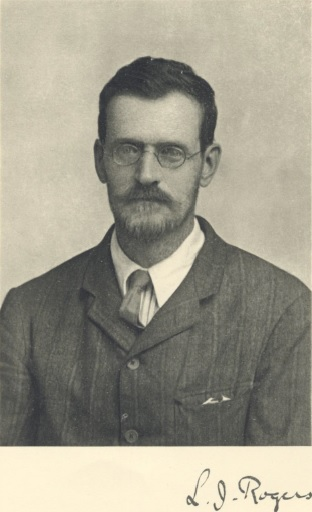
\includegraphics[height=0.4\textwidth]{Rogers.jpg}
    \end{center}
    \textbf{Leonard James Rogers} (30 March 1862, Oxford, England, – 12 September 1933, Oxford, England) was a British mathematician who was the first to discover the Rogers–Ramanujan identity and Hölder's inequality, and who introduced Rogers polynomials. The Rogers–Szegő polynomials are named after him.
\end{qte}

Rogers published his result in \textit{"An extension of a certain theorem in inequalities"} in 1888 starting with the extended AM-GM inequality:

\begin{thm}{Extended AM-GM inequality}{ext}
    Let $a_i, b_i$ be positive for all $i \in [n]$, then
    \begin{math}
        (\frac{\sum a_i b_i}{\sum a_i})^{\sum a_i} \ge \prod b_i^{a_i}
    .\end{math}
\end{thm}

Here is the proof in his paper:

\begin{proof}[Proof]
    ~
    \begin{itemize}
        \item Firstly, let $a_i$ be integers, then it can be considered as \rf{ag} with each $b_i$ occurring $a_i$ times.
        \item Then, if $a_i$ are rational numbers, we can also multiply with the least common multiple of denominators of $a_i$. Then it becomes the first situation.
        \item Finally, as for real numbers, we can always use fractions to approximate them with arbitrary precision. Thus we can substitute real numbers with fractions and then apply the second case. \textit{(Can this really work? I kind of doubt it.)} Here is the original text:
            \begin{qte}
                Then we may substitute for each of these quantities fractions, which may differ from them by less than any assigned quantities, and since the theorem is tru for the substituted fractions, we may assume it also true for the given incommensurables.
            \end{qte}
    \end{itemize}
\end{proof}

Then, with the help with this inequality, Rogers proposed:
\begin{thm}{Rogers' inequality}{ro}
    If $0 < t < r < m$ and $a_i, b_i$ are positive for all $i \in [n]$, then
    \begin{math}
        (\sum a_i b_i^m)^{r-t} (\sum a_ib_i^r)^{m-r} \ge (\sum a_i b_i^r)^{m-t}
    .\end{math}
\end{thm}

\begin{proof}[Proof]
    Let $S_k = \sum a_i b_i^k$, $0 < t < r < m$, and substitute $a_i$ in \rf{ext} with $a_i b_i^r$, $b_i$ with $b_i^{m-r}$:
    \begin{math}
        (\frac{S_m}{S_r})^{S_r} \ge \prod (b_i^{m-r})^{a_i b_i^t} = (\prod b_i^{a_i b_i^r})^{m-r}
    .\end{math}

    Then we substitute $a_i$ with $a_i b_i^r$, while $b_i$ becomes $b_i^{t-r}$:
    \begin{math}
        (\frac{S_t}{S_r})^{S_r} \ge (\prod b_i^{a_i b_i^r})^{t-r} \iff
        (\frac{S_r}{S_t})^{S_r} \le (\prod b_i^{a_i b_i^r})^{r-t}
    .\end{math}

    Combine the two parts, we can get
    \begin{math}
        (\frac{S_m}{S_r})^{\frac{S_r}{m-r}} \ge \prod b_i^{a_i b_i^r} \ge (\frac{S_r}{S_t})^\frac{S_r}{r-t}
    .\end{math}

    And it can be simplified to
    \begin{math}
        S_m^{r-t} \cdot S_t^{m-r} \ge S_r^{m-t}
    .\end{math}
\end{proof}

\section{Hölder and his inequality}

\begin{qte}
    \begin{center}
        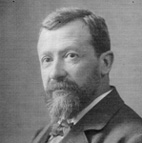
\includegraphics[height=0.3\textwidth]{Hoelder.jpg}
    \end{center}

    \textbf{Otto Ludwig Hölder} (December 22, 1859 – August 29, 1937) was a German mathematician born in Stuttgart.

Hölder first studied at the Polytechnikum (which today is the University of Stuttgart) and then in 1877 went to Berlin where he was a student of Leopold Kronecker, Karl Weierstrass, and Ernst Kummer.

He is noted for many theorems including: Hölder's inequality, the Jordan–Hölder theorem, the theorem stating that every linearly ordered group that satisfies an Archimedean property is isomorphic to a subgroup of the additive group of real numbers, the classification of simple groups of order up to 200, the anomalous outer automorphisms of the symmetric group S6, and Hölder's theorem, which implies that the Gamma function satisfies no algebraic differential equation. Another idea related to his name is the Hölder condition (or Hölder continuity) which is used in many areas of analysis, including the theories of partial differential equations and function spaces.
\end{qte}

Hölder introduced the inequality in his paper \textit{"Ueber einen Mittelwerthssatz"} in 1889:

\begin{qte}
    Bedeutet nämlich $\phi (x)$ eine Function einer reellen Veränderlichen mit zunehmendem Differentialguotienten, so ist das arithmetische Mittel aus einer beliebigen Zahl von Functionswerthen stets
größer als der Functionswerth, welcher dem in derselben Weise gebildeten Mittelwerth der zugehörigen Argumente entspricht. Dabei ist der Begriff des arithmetischen Mittels gleich in der allgemeinen Weise zu nehmen, daß jedem der Werthe, aus welchen dasselbe zu bilden ist, eine beliebige positive Größe als Gewicht zugeordnet wird, so daß also die Formel
\begin{math}
    \frac{a_1 \phi (x_1) + a_2\phi (x_2) + \cdots + a_n \phi (x_n)}{a_1 + a_2 + \cdots + a_n} > \phi (\frac{a_1 x_1 + a_2x_2 + \cdots  + a_n x_n}{a_1 + a_2 + \cdots  + a_n})
.\end{math}
den Ausdruck des genannten Satzes darstellt.
\end{qte}

I do not know much about German, but with the help of Google translation, the main idea may be:

\begin{thm}{Inequality}{jen}
    Let $\phi $ be a convex function and $a_i > 0,  x_i > 0$ for all $i \in [n]$, then there holds the inequality:
\begin{math}
    \frac{\sum a_i \phi (x_i)}{\sum a_i} \ge \phi (\frac{\sum a_i x_i}{\sum a_i})
.\end{math}
\end{thm}

The original proof is omitted because it was totally written in German. I would like to consider it as an extended version of Jensen's inequality. (But note that Jensen's inequality was proposed in 1906, later than this paper.)

In section 7, 8, 9, 10, Hölder gave some applications with \rf{jen}.

Let $\phi (x) = x^m(m > 1)$, we have $\phi ''(x) = m(m-1)x^{m-2} > 0$. Thus
\begin{thm}{Inequality}{ho}
    Let $a_i > 0,  x_i > 0$ for all $i \in [n]$ and $m > 1$, then:
    \begin{math}
        (\sum a_i)^{m-1} \cdot (\sum a_i x_i^m) \ge (\sum a_i x_i)^m
    .\end{math}
\end{thm}

This is actually \rf{ro} when $r = 1, t = 0$.

We can also let $\phi (x) = \e^x$, $y_i = \e^{x_i}$, resulting in
\begin{math}
    (\frac{\sum a_i y_i}{\sum a_i})^{\sum a_i} \ge \prod y_i^{a_i}
.\end{math}

This is exactly the result('Ausgangspunkt', starting point) in Rogers' paper. Hölder even mentioned this result of Rogers' here!
\begin{qte}
    Dies ist der Satz vom arithmetischen und geometrischen Mittel in seiner allgemeinsten Gestalt, wie ihn Herr Rogers zum Ausgangspunkt wählt, 1(1).
\end{qte}

\section{Relationship between the inequalities}

The inequalities above all have similar forms, so I think they might be equivalent.

\begin{thm}{Theorem}{}
    \rf{well} $\iff$ \rf{ho}.
\end{thm}

\begin{proof}[Proof]
    ~
    \begin{itemize}
        \item $\impliedby$: Note that the second term in \rf{ho} have $a_i$ as well as $x_i$, so we can try to let $a_ix_i = a_i^s \cdot (a_i^{1-s}x_i)$ in order to eliminate $a_i$.
            \begin{math}
                \sum a_i x_i &= \sum a_i^s (a_i^{1-s} x_i) \\
                \text{ (by \rf{ho}) } &\le (\sum a_i^s)^\frac{m-1}{m} (\sum a_i^s \cdot a_i^{m(1-s)} x_i^m)^\frac{1}{m}
            .\end{math}

            Solve $s + m(1-s) = 0$ and we have $s = \frac{m}{m-1}$. Thus
            \begin{math}
                \sum a_i x_i \le (\sum a_i^\frac{m}{m-1})^\frac{m-1}{m} (\sum x_i^m)^\frac{1}{m}
            .\end{math}

            In this case, $p = \frac{m}{m-1}, q = m$ and every pair $(p, q)$ can be reached with $m = q > 1$.

        \item $\implies $: Similarly, 
            \begin{math}
                (\sum a_i x_i)^m &= (\sum a_i^s a_i^{1-s} x_i)^m \\
                \text{ (by \rf{well}) }&\le (\sum a_i^{ps})^\frac{m}{p} (\sum (a_i^{1-s}x_i)^\frac{p}{p-1})^\frac{m(p-1)}{p}
            .\end{math}

            Let $s = \frac{1}{p}$, $p = \frac{m}{m-1}$, then
            \begin{math}
                (\sum a_i x_i)^m \le (\sum a_i)^{m-1} (\sum a_i x_i^m)
            .\end{math}

            Every $m > 1$ can be reached by letting $p = \frac{m}{m-1} > 1$.
    \end{itemize}
\end{proof}

\rf{ro} and \rf{ho} seems similar, but more complicated. I think \rf{ro} and \rf{well} might be also equivalent, and that's why we can say Rogers and Hölder actually proposed the same inequality.

\section{Stigler's law of eponymy}

Like Hölder's inequality, it is not rare for a theorem not to be named after its first discoverer. Actually, Stephen Stigler in his 1980 publication proposed \textit{Stigler's law of eponymy}\footnote{from Greek epōnumos "given as a name, giving one's name to something," as a plural noun (short for eponymoi heroes) denoting founders (legendary or real) of tribes, cities, etc.; from combining form of epi "upon, (called) after," + onyma, Aeolic dialectal variant of onoma "name".}, which states that \textit{no scientific discovery is named after its original discoverer}. As Mark Twain said,
\begin{qte}
    It takes a thousand men to invent a telegraph, or a steam engine, or a phonograph, or a photograph, or a telephone or any other important thing — and the last man gets the credit and we forget the others. He added his little mite — that is all he did. These object lessons should teach us that ninety-nine parts of all things that proceed from the intellect are plagiarisms, pure and simple; and the lesson ought to make us modest. But nothing can do that.
\end{qte}

Famous theorems including \textit{Chebyshev's inequality, Burnside's lemma, Cayley–Hamilton theorem, L'Hôpital's rule, Zorn's lemma} are also misnamed, see \url{https://en.wikipedia.org/wiki/List_of_misnamed_theorems} and \url{https://en.wikipedia.org/wiki/List_of_examples_of_Stigler%27s_law}.

\section{Conclusion}

Rogers introduced the inequality in 1888. Hölder, knowing the work of Rogers', introduced another (strengthened?) version of it in 1889. This result is now known as Hölder's inequality.

\section*{Reference}

\begin{itemize}
    \item Wikipedia, Hölder's inequality, \url{https://en.wikipedia.org/wiki/Hölder%27s_inequality}.
    \item Rogers, L. J. (February 1888), "An extension of a certain theorem in inequalities", Messenger of Mathematics, New Series, XVII (10): 145–150, JFM 20.0254.02.
    \item Hölder, O. (1889), "Ueber einen Mittelwertsatz", Nachrichten von der Königl. Gesellschaft der Wissenschaften und der Georg-Augusts-Universität zu Göttingen, Band (in German), 1889 (2): 38–47, JFM 21.0260.07.
    \item Wikipedia, Leonard James Rogers, \url{https://en.wikipedia.org/wiki/Leonard_James_Rogers}.
    \item Wikipedia, Otto Hölder, \url{https://en.wikipedia.org/wiki/Otto_Hölder}.
    \item Wikipedia, Stigler's law of eponymy, \url{https://en.wikipedia.org/wiki/Stigler%27s_law_of_eponymy}.
    \item Wikipedia, List of misnamed theorems, \url{https://en.wikipedia.org/wiki/List_of_misnamed_theorems}.
    \item Wikipedia, List of examples of Stigler's law, \url{https://en.wikipedia.org/wiki/List_of_examples_of_Stigler%27s_law}.
\end{itemize}

\end{document}
